\documentclass[11pt, oneside]{article}
\usepackage[letterpaper, margin=2cm]{geometry}
\usepackage{MATH566}
%\usepackage{sagetex}

\begin{document}
\noindent \textbf{\Large{Caleb Logemann \\
MATH 566 Discrete Optimization\\
Homework 10
}}

%\lstinputlisting[language=Sage]{03_2.sage}
\begin{enumerate}
  \item % #1
    Solve the following problem using branch and bound.
    Draw the branching tree too.
    \[
      (P)=
      \begin{cases}
        \text{maximize} & -x_1 + 4x_2\\
        \text{subject to} & -10x_1 + 20x_2 \leq 22 \\
                          &   5x_1 +10x_2 \leq 49 \\
                          &  x_1 \leq 5\\
                          & x_i \geq 0,  x_i \in \mathbb{Z} \text{ for } i \in \{1,2\}
      \end{cases}
    \]
    You can use any linear programming solver for solving the relaxations.

  \item % #2
    Let $P$ be a convex hull of $(0,0), (0,1), (k,\frac{1}{2})$.
    Give an upper bound on Chv\'atal's rank of $P$.
    (Show it is at most $2k$, actually, it is exactly $2k$.)\\
    % Hints: Write $P$ as an intersection of half-spaces, use \emph{induction}
    % on $k$. See what we were doing in notes.}\\
    Drawing of $P$ for $k=3$.
    \begin{center}
      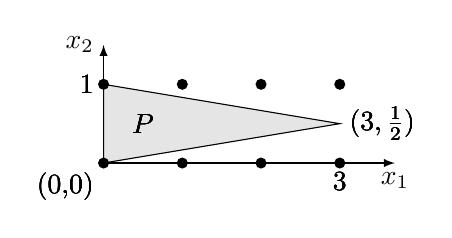
\begin{tikzpicture}[scale=1]
        \draw[fill=gray!20]
          (0,0) -- (3,0.5) -- (0,1) -- cycle
        ;
        \foreach \x in {0,1,2,3}{
          \foreach \y in {0,1}{
            \fill (\x,\y) circle(2 pt);
        }
        \draw
          (0,0) node[below left]{(0,0)}
          (0,1) node[left]{1}
          (3,0) node[below]{3}
          (3,0.5) node[right]{$(3,\frac{1}{2})$}
        ;
        \draw
          (0.5,0.5) node{$P$}
        ;
        }
        \draw[-latex](0,0) -- (3.7,0) node[below]{$x_1$};
        \draw[-latex](0,0) -- (0,1.5) node[left]{$x_2$};
      \end{tikzpicture}
    \end{center}

  \item % #3 Done
    Run Edmond's Blossom algorithm on the following graph. Notice that somebody
    already found a partial matching. What is the largest possible matching?
    Try to start growing augmenting tree from $x$, use BFS algorithm for building the tree.
    \begin{center}
      \tikzset{insep/.style={inner sep=2.2pt, outer sep=0pt, circle, fill},}
      \begin{tikzpicture}[scale=1.5]
        \draw   
          (0,0) node[insep,label=left: ](a){} 
          (1,0) node[insep,label=left: ](b){}
          ++(72:1) node[insep,label=left: ](c){}
          ++(144:1) node[insep,label=left: ](d){}
          ++(216:1) node[insep,label=left: ](e){}
          (b) ++ (-72:1) node[insep,label=left: ](g){}  
          ++(-144:1) node[insep,label=left: ](i){}
          ++(-216:1) node[insep,label=left: ](j){}
          (c) ++(1,0) node[insep,label=left: ](f){} 
          (g) ++(1,0) node[insep,label=left: ](h){} 
          (d) ++ (3,0) node[insep,label=left: ](k){}
          (i) ++ (3,0) node[insep,label=left: ](l){}
          (b) ++ (3.5,0) node[insep,label=left: ](m){}
          (d) ++ (-3,0) node[insep,label=left: ](n){}
          (i) ++ (-3,0) node[insep,label=left: ](o){}
          (a) ++ (-3.5,0) node[insep,label=left:$x$](p){}
        ;
        \draw
          (a)--(b) (a)--(e) (a)--(j) (b)--(g)--(h) (g)--(i)
          (n)--(d)--(k)--(m)--(l)--(i)--(o)--(p)--(n) (n)--(o)
          (d)--(c)--(f) (k)--(l)
        ;
        \draw[line width=2.5pt]
          (n)--(o) (e)--(d) (i)--(j) (b)--(c) (f)--(h) 
        ;
        \draw[dashed]
        ;
      \end{tikzpicture}
    \end{center}

    First I will label all of the vertices of the graph as follows.
    \begin{center}
      \tikzset{insep/.style={inner sep=2.2pt, outer sep=0pt, circle, fill},}
      \begin{tikzpicture}[scale=1.4]
        \draw   
          (0,0) node[insep,label=left:a](a){} 
          (1,0) node[insep,label=right:b](b){}
          ++(72:1) node[insep,label=left:c](c){}
          ++(144:1) node[insep,label=above:d](d){}
          ++(216:1) node[insep,label=left:e](e){}
          (b) ++ (-72:1) node[insep,label=left:g](g){}  
          ++(-144:1) node[insep,label=below:i](i){}
          ++(-216:1) node[insep,label=left:j](j){}
          (c) ++(1,0) node[insep,label=above:f](f){} 
          (g) ++(1,0) node[insep,label=below:h](h){} 
          (d) ++ (3,0) node[insep,label=above:k](k){}
          (i) ++ (3,0) node[insep,label=below:l](l){}
          (b) ++ (3.5,0) node[insep,label=right:m](m){}
          (d) ++ (-3,0) node[insep,label=above:n](n){}
          (i) ++ (-3,0) node[insep,label=below:o](o){}
          (a) ++ (-3.5,0) node[insep,label=left:$x$](p){}
        ;
        \draw
          (a)--(b) (a)--(e) (a)--(j) (b)--(g)--(h) (g)--(i)
          (n)--(d)--(k)--(m)--(l)--(i)--(o)--(p)--(n) (n)--(o)
          (d)--(c)--(f) (k)--(l)
        ;
        \draw[line width=2.5pt]
          (n)--(o) (e)--(d) (i)--(j) (b)--(c) (f)--(h) 
        ;
        \draw[dashed]
        ;
      \end{tikzpicture}
    \end{center}

    The first step in the algorithm is to grow forest from the exposed vertices.
    The following is the forest created by adding edges $(x, n)$ and $(x, o)$,
    which results in a blossom.
    \begin{center}
      \tikzset{insep/.style={inner sep=2.2pt, outer sep=0pt, circle, fill},}
      \begin{tikzpicture}[scale=1.4]
        \draw
          (0,0) node[insep,label=above:x](x){}
          (-.5,-1) node[insep,label=left:n](n){}
          (.5,-1) node[insep,label=right:o](o){}
          (1,0) node[insep,label=above:a](a){}
          (2,0) node[insep,label=above:g](g){}
          (3,0) node[insep,label=above:k](k){}
          (4,0) node[insep,label=above:l](l){}
          (5,0) node[insep,label=above:m](m){}
        ;
        \draw
          (x) -- (n)
          (x) -- (o)
        ;
        \draw[line width=2.5pt]
          (n) -- (o)
        ;
      \end{tikzpicture}
    \end{center}
    The blossom needs to be contracted in the forest and the graph.
    The contracted graph and forest are shown below.
    \begin{center}
      \tikzset{insep/.style={inner sep=2.2pt, outer sep=0pt, circle, fill},}
      \begin{tikzpicture}[scale=1.4]
        \draw   
          (0,0) node[insep,label=left:a](a){} 
          (1,0) node[insep,label=right:b](b){}
          ++(72:1) node[insep,label=left:c](c){}
          ++(144:1) node[insep,label=above:d](d){}
          ++(216:1) node[insep,label=left:e](e){}
          (b) ++ (-72:1) node[insep,label=left:g](g){}  
          ++(-144:1) node[insep,label=below:i](i){}
          ++(-216:1) node[insep,label=left:j](j){}
          (c) ++(1,0) node[insep,label=above:f](f){} 
          (g) ++(1,0) node[insep,label=below:h](h){} 
          (d) ++ (3,0) node[insep,label=above:k](k){}
          (i) ++ (3,0) node[insep,label=below:l](l){}
          (b) ++ (3.5,0) node[insep,label=right:m](m){}
          %(d) ++ (-3,0) node[insep,label=above:n](n){}
          %(i) ++ (-3,0) node[insep,label=below:o](o){}
          (a) ++ (-3.5,0) node[insep,label=left:$x$](p){}
        ;
        \draw
          (a)--(b) (a)--(e) (a)--(j) (b)--(g)--(h) (g)--(i)
          (p)--(d)--(k)--(m)--(l)--(i)--(p)
          (d)--(c)--(f) (k)--(l)
        ;
        \draw[line width=2.5pt]
          (e)--(d) (i)--(j) (b)--(c) (f)--(h) 
        ;
        \draw[dashed]
        ;
      \end{tikzpicture}
    \end{center}
    \begin{center}
      \tikzset{insep/.style={inner sep=2.2pt, outer sep=0pt, circle, fill},}
      \begin{tikzpicture}[scale=1.4]
        \draw
          (0,0) node[insep,label=above:x](x){}
          (1,0) node[insep,label=above:a](a){}
          (2,0) node[insep,label=above:g](g){}
          (3,0) node[insep,label=above:k](k){}
          (4,0) node[insep,label=above:l](l){}
          (5,0) node[insep,label=above:m](m){}
        ;
        \draw
        ;
        \draw[line width=2.5pt]
        ;
      \end{tikzpicture}
    \end{center}
    This tree can now be continued to be expanded by adding $(x, i)$ and
    $(x, d)$ which causes $(i, j)$ and $(d, e)$ to be added respectively.
    Now adding the edge $(j, a)$ creates an augmenting path.
    The alternating forest is now
    \begin{center}
      \tikzset{insep/.style={inner sep=2.2pt, outer sep=0pt, circle, fill},}
      \begin{tikzpicture}[scale=1.4]
        \draw
          (0,0) node[insep,label=above:x](x){}
          (.5,-1) node[insep,label=left:i](i){}
          (.5,-2) node[insep,label=right:j](j){}
          (-.5,-1) node[insep,label=left:d](d){}
          (-.5,-2) node[insep,label=left:e](e){}
          (1,0) node[insep,label=above:a](a){}
          (2,0) node[insep,label=above:g](g){}
          (3,0) node[insep,label=above:k](k){}
          (4,0) node[insep,label=above:l](l){}
          (5,0) node[insep,label=above:m](m){}
        ;
        \draw
          (x) -- (i)
          (x) -- (d)
          (j) -- (a)
        ;
        \draw[line width=2.5pt]
          (i) -- (j)
          (d) -- (e)
        ;
      \end{tikzpicture}
    \end{center}

    This augmenting path going around the blossom is $x\to n\to o\to i\to j\to a$.
    Doing the augmentation addes $(x,n)$,$(o,i)$, and $(j,a)$ to the matching,
    while removing $(n,o)$ and $(i, j)$.
    The new matching is shown in the following graph.
    \begin{center}
      \tikzset{insep/.style={inner sep=2.2pt, outer sep=0pt, circle, fill},}
      \begin{tikzpicture}[scale=1.4]
        \draw
          (0,0) node[insep,label=left:a](a){} 
          (1,0) node[insep,label=right:b](b){}
          ++(72:1) node[insep,label=left:c](c){}
          ++(144:1) node[insep,label=above:d](d){}
          ++(216:1) node[insep,label=left:e](e){}
          (b) ++ (-72:1) node[insep,label=left:g](g){}  
          ++(-144:1) node[insep,label=below:i](i){}
          ++(-216:1) node[insep,label=left:j](j){}
          (c) ++(1,0) node[insep,label=above:f](f){} 
          (g) ++(1,0) node[insep,label=below:h](h){} 
          (d) ++ (3,0) node[insep,label=above:k](k){}
          (i) ++ (3,0) node[insep,label=below:l](l){}
          (b) ++ (3.5,0) node[insep,label=right:m](m){}
          (d) ++ (-3,0) node[insep,label=above:n](n){}
          (i) ++ (-3,0) node[insep,label=below:o](o){}
          (a) ++ (-3.5,0) node[insep,label=left:$x$](p){}
        ;
        \draw
          (a)--(b) (a)--(e) (a)--(j) (b)--(g)--(h) (g)--(i)
          (n)--(d)--(k)--(m)--(l)--(i)--(o) (n)--(o)
          (d)--(c)--(f) (k)--(l)
          (n)--(o)
          (i)--(j)
          (p)--(o)
        ;
        \draw[line width=2.5pt]
        (e)--(d) (b)--(c) (f)--(h) (p)--(n) (o)--(i) (j)--(a)
        ;
        \draw[dashed]
        ;
      \end{tikzpicture}
    \end{center}

    Again in order to find an augmeting path we start growing the alternating
    forest from the exposed vertices.
    Note that an augmenting path can be found directly by adding $(l, m)$.
    \begin{center}
      \tikzset{insep/.style={inner sep=2.2pt, outer sep=0pt, circle, fill},}
      \begin{tikzpicture}[scale=1.4]
        \draw
          (2,0) node[insep,label=above:g](g){}
          (3,0) node[insep,label=above:k](k){}
          (4,0) node[insep,label=above:l](l){}
          (5,0) node[insep,label=above:m](m){}
        ;
        \draw
          (l) -- (m)
        ;
        \draw[line width=2.5pt]
        ;
      \end{tikzpicture}
    \end{center}
    Augmenting on this path adds $(l, m)$ to the matching, so the new matching is
    \begin{center}
      \tikzset{insep/.style={inner sep=2.2pt, outer sep=0pt, circle, fill},}
      \begin{tikzpicture}[scale=1.4]
        \draw
          (0,0) node[insep,label=left:a](a){} 
          (1,0) node[insep,label=right:b](b){}
          ++(72:1) node[insep,label=left:c](c){}
          ++(144:1) node[insep,label=above:d](d){}
          ++(216:1) node[insep,label=left:e](e){}
          (b) ++ (-72:1) node[insep,label=left:g](g){}  
          ++(-144:1) node[insep,label=below:i](i){}
          ++(-216:1) node[insep,label=left:j](j){}
          (c) ++(1,0) node[insep,label=above:f](f){} 
          (g) ++(1,0) node[insep,label=below:h](h){} 
          (d) ++ (3,0) node[insep,label=above:k](k){}
          (i) ++ (3,0) node[insep,label=below:l](l){}
          (b) ++ (3.5,0) node[insep,label=right:m](m){}
          (d) ++ (-3,0) node[insep,label=above:n](n){}
          (i) ++ (-3,0) node[insep,label=below:o](o){}
          (a) ++ (-3.5,0) node[insep,label=left:$x$](p){}
        ;
        \draw
          (a)--(b)
          (a)--(e)
          (a)--(j)
          (b)--(g)--(h)
          (g)--(i)
          (n)--(d)--(k)--(m)--(l)--(i)--(o)
          (n)--(o)
          (d)--(c)--(f)
          (k)--(l)
          (n)--(o)
          (i)--(j)
          (p)--(o)
        ;
        \draw[line width=2.5pt]
          (e)--(d)
          (b)--(c)
          (f)--(h)
          (p)--(n)
          (o)--(i)
          (j)--(a)
          (l)--(m)
        ;
        \draw[dashed]
        ;
      \end{tikzpicture}
    \end{center}

    We now have only two exposed vertices, so the alternating forest needs to be
    grown to check if there is an augmenting path from $g$ to $k$.
    Adding the edges incident to $g$ and $k$ results in the following.
    \begin{center}
      \tikzset{insep/.style={inner sep=2.2pt, outer sep=0pt, circle, fill},}
      \begin{tikzpicture}[scale=1.4]
        \draw
          (1,0) node[insep,label=above:g](g){}
          (0,-1) node[insep,label=left:b](b){}
          (0,-2) node[insep,label=left:c](c){}
          (1,-1) node[insep,label=left:h](h){}
          (1,-2) node[insep,label=left:f](f){}
          (2,-1) node[insep,label=right:i](i){}
          (2,-2) node[insep,label=right:o](o){}
          (4,0) node[insep,label=above:k](k){}
          (3,-1) node[insep,label=left:l](l){}
          (4,-1) node[insep,label=right:m](m){}
          (5,-1) node[insep,label=right:d](d){}
          (5,-2) node[insep,label=right:e](e){}
        ;
        \draw
          (g)--(b)
          (g)--(h)
          (g)--(i)
          (k)--(l)
          (k)--(m)
          (k)--(d)
        ;
        \draw[line width=2.5pt]
          (l)--(m)
          (b)--(c)
          (h)--(f)
          (i)--(o)
          (d)--(e)
        ;
      \end{tikzpicture}
    \end{center}
    There is a blossom containing $k$, $l$, and $m$.
    Contracting this blossom in the forest and the graph results in
    \begin{center}
      \tikzset{insep/.style={inner sep=2.2pt, outer sep=0pt, circle, fill},}
      \begin{tikzpicture}[scale=1.4]
        \draw
          (0,0) node[insep,label=left:a](a){} 
          (1,0) node[insep,label=right:b](b){}
          ++(72:1) node[insep,label=left:c](c){}
          ++(144:1) node[insep,label=above:d](d){}
          ++(216:1) node[insep,label=left:e](e){}
          (b) ++ (-72:1) node[insep,label=left:g](g){}  
          ++(-144:1) node[insep,label=below:i](i){}
          ++(-216:1) node[insep,label=left:j](j){}
          (c) ++(1,0) node[insep,label=above:f](f){} 
          (g) ++(1,0) node[insep,label=below:h](h){} 
          (d) ++ (3,0) node[insep,label=above:k](k){}
          (d) ++ (-3,0) node[insep,label=above:n](n){}
          (i) ++ (-3,0) node[insep,label=below:o](o){}
          (a) ++ (-3.5,0) node[insep,label=left:$x$](p){}
        ;
        \draw
          (a)--(b)
          (a)--(e)
          (a)--(j)
          (b)--(g)--(h)
          (g)--(i)
          (n)--(d)
          (d)--(k)
          (k) to[out=-90, in=0, distance=100] (i)
          (i)--(o)
          (n)--(o)
          (d)--(c)--(f)
          (n)--(o)
          (i)--(j)
          (p)--(o)
        ;
        \draw[line width=2.5pt]
          (e)--(d)
          (b)--(c)
          (f)--(h)
          (p)--(n)
          (o)--(i)
          (j)--(a)
        ;
        \draw[dashed]
        ;
      \end{tikzpicture}
    \end{center}
    \begin{center}
      \tikzset{insep/.style={inner sep=2.2pt, outer sep=0pt, circle, fill},}
      \begin{tikzpicture}[scale=1.4]
        \draw
          (1,0) node[insep,label=above:g](g){}
          (0,-1) node[insep,label=left:b](b){}
          (0,-2) node[insep,label=left:c](c){}
          (1,-1) node[insep,label=left:h](h){}
          (1,-2) node[insep,label=left:f](f){}
          (2,-1) node[insep,label=right:i](i){}
          (2,-2) node[insep,label=right:o](o){}
          (3,0) node[insep,label=above:{(k,l,m)}](k){}
          (3,-1) node[insep,label=right:d](d){}
          (3,-2) node[insep,label=right:e](e){}
        ;
        \draw
          (g)--(b)
          (g)--(h)
          (g)--(i)
          (k)--(d)
        ;
        \draw[line width=2.5pt]
          (b)--(c)
          (h)--(f)
          (i)--(o)
          (d)--(e)
        ;
      \end{tikzpicture}
    \end{center}
    Now let us add $(c, f)$, this creates a blossom of length 5.
    \begin{center}
      \tikzset{insep/.style={inner sep=2.2pt, outer sep=0pt, circle, fill},}
      \begin{tikzpicture}[scale=1.4]
        \draw
          (1,0) node[insep,label=above:g](g){}
          (0,-1) node[insep,label=left:b](b){}
          (0,-2) node[insep,label=left:c](c){}
          (1,-1) node[insep,label=left:h](h){}
          (1,-2) node[insep,label=right:f](f){}
          (2,-1) node[insep,label=right:i](i){}
          (2,-2) node[insep,label=right:o](o){}
          (3,0) node[insep,label=above:{(k,l,m)}](k){}
          (3,-1) node[insep,label=right:d](d){}
          (3,-2) node[insep,label=right:e](e){}
        ;
        \draw
          (g)--(b)
          (g)--(h)
          (g)--(i)
          (k)--(d)
          (c)--(f)
        ;
        \draw[line width=2.5pt]
          (b)--(c)
          (h)--(f)
          (i)--(o)
          (d)--(e)
        ;
      \end{tikzpicture}
    \end{center}
    Contracting this blossom in the forest and graph results in
    \begin{center}
      \tikzset{insep/.style={inner sep=2.2pt, outer sep=0pt, circle, fill},}
      \begin{tikzpicture}[scale=1.4]
        \draw
          (0,0) node[insep,label=left:a](a){} 
          ++(108:1) node[insep,label=left:e](e){}
          ++(36:1) node[insep,label=above:d](d){}
          (a) ++(-108:1) node[insep,label=left:j](j){}
          ++(-36:1) node[insep,label=below:i](i){}
          (1,0) node[insep,label=right:g](g){}
          (d) ++ (3,0) node[insep,label=above:k](k){}
          (d) ++ (-3,0) node[insep,label=above:n](n){}
          (i) ++ (-3,0) node[insep,label=below:o](o){}
          (a) ++ (-3.5,0) node[insep,label=left:$x$](p){}
        ;
        \draw
          (a)--(g)
          (a)--(e)
          (a)--(j)
          (g)--(i)
          (n)--(d)
          (d)--(k)
          (k) to[out=-90, in=0, distance=100] (i)
          (i)--(o)
          (n)--(o)
          (d)--(g)
          (n)--(o)
          (i)--(j)
          (p)--(o)
        ;
        \draw[line width=2.5pt]
          (e)--(d)
          (p)--(n)
          (o)--(i)
          (j)--(a)
        ;
        \draw[dashed]
        ;
      \end{tikzpicture}
    \end{center}
    \begin{center}
      \tikzset{insep/.style={inner sep=2.2pt, outer sep=0pt, circle, fill},}
      \begin{tikzpicture}[scale=1.4]
        \draw
          (1,0) node[insep,label=above:{(g,b,c,f,h)}](g){}
          (1,-1) node[insep,label=right:i](i){}
          (1,-2) node[insep,label=right:o](o){}
          (3,0) node[insep,label=above:{(k,l,m)}](k){}
          (3,-1) node[insep,label=right:d](d){}
          (3,-2) node[insep,label=right:e](e){}
        ;
        \draw
          (g)--(i)
          (k)--(d)
        ;
        \draw[line width=2.5pt]
          (i)--(o)
          (d)--(e)
        ;
      \end{tikzpicture}
    \end{center}
    We can now continue growing the forest, consider adding $(e, a)$ and $(o, x)$.
    \begin{center}
      \tikzset{insep/.style={inner sep=2.2pt, outer sep=0pt, circle, fill},}
      \begin{tikzpicture}[scale=1.4]
        \draw
          (1,0) node[insep,label=above:{(g,b,c,f,h)}](g){}
          (1,-1) node[insep,label=right:i](i){}
          (1,-2) node[insep,label=right:o](o){}
          (1, -3) node[insep,label=right:x](x){}
          (1, -4) node[insep,label=right:n](n){}
          (3,0) node[insep,label=above:{(k,l,m)}](k){}
          (3,-1) node[insep,label=right:d](d){}
          (3,-2) node[insep,label=right:e](e){}
          (3,-3) node[insep,label=right:a](a){}
          (3,-4) node[insep,label=right:j](j){}
        ;
        \draw
          (g)--(i)
          (k)--(d)
          (o)--(x)
          (e)--(a)
        ;
        \draw[line width=2.5pt]
          (i)--(o)
          (d)--(e)
          (x)--(n)
          (a)--(j)
        ;
      \end{tikzpicture}
    \end{center}
    The edges $(g, a)$, $(k, i)$, $(j, i)$ and $(n, d)$ can't be added because
    they connect to vertices that are an odd distance from their root.
    The last edge that can be added is $(n,o)$.
    This creates a blossom, but as it is the last edge that can be added and
    no augmenting path has been found, we can conclude that we have found the
    maximal matching.
    The final forest and maximal matching are
    \begin{center}
      \tikzset{insep/.style={inner sep=2.2pt, outer sep=0pt, circle, fill},}
      \begin{tikzpicture}[scale=1.4]
        \draw
          (1,0) node[insep,label=above:{(g,b,c,f,h)}](g){}
          (1,-1) node[insep,label=right:i](i){}
          (1,-2) node[insep,label=right:o](o){}
          (1, -3) node[insep,label=right:x](x){}
          (1, -4) node[insep,label=right:n](n){}
          (3,0) node[insep,label=above:{(k,l,m)}](k){}
          (3,-1) node[insep,label=right:d](d){}
          (3,-2) node[insep,label=right:e](e){}
          (3,-3) node[insep,label=right:a](a){}
          (3,-4) node[insep,label=right:j](j){}
        ;
        \draw
          (g)--(i)
          (k)--(d)
          (o)--(x)
          (e)--(a)
          (n) to[out=180, in=180] (o)
        ;
        \draw[line width=2.5pt]
          (i)--(o)
          (d)--(e)
          (x)--(n)
          (a)--(j)
        ;
      \end{tikzpicture}
    \end{center}
    \begin{center}
      \tikzset{insep/.style={inner sep=2.2pt, outer sep=0pt, circle, fill},}
      \begin{tikzpicture}[scale=1.4]
        \draw
          (0,0) node[insep,label=left:a](a){} 
          (1,0) node[insep,label=right:b](b){}
          ++(72:1) node[insep,label=left:c](c){}
          ++(144:1) node[insep,label=above:d](d){}
          ++(216:1) node[insep,label=left:e](e){}
          (b) ++ (-72:1) node[insep,label=left:g](g){}  
          ++(-144:1) node[insep,label=below:i](i){}
          ++(-216:1) node[insep,label=left:j](j){}
          (c) ++(1,0) node[insep,label=above:f](f){} 
          (g) ++(1,0) node[insep,label=below:h](h){} 
          (d) ++ (3,0) node[insep,label=above:k](k){}
          (i) ++ (3,0) node[insep,label=below:l](l){}
          (b) ++ (3.5,0) node[insep,label=right:m](m){}
          (d) ++ (-3,0) node[insep,label=above:n](n){}
          (i) ++ (-3,0) node[insep,label=below:o](o){}
          (a) ++ (-3.5,0) node[insep,label=left:$x$](p){}
        ;
        \draw
          (a)--(b)
          (a)--(e)
          (a)--(j)
          (b)--(g)--(h)
          (g)--(i)
          (n)--(d)--(k)--(m)--(l)--(i)--(o)
          (n)--(o)
          (d)--(c)--(f)
          (k)--(l)
          (n)--(o)
          (i)--(j)
          (p)--(o)
        ;
        \draw[line width=2.5pt]
          (e)--(d)
          (b)--(c)
          (f)--(h)
          (p)--(n)
          (o)--(i)
          (j)--(a)
          (l)--(m)
        ;
        \draw[dashed]
        ;
      \end{tikzpicture}
    \end{center}

    Therefore the largest possible matching contains 7 edges.

  \item % #4 Done
    Find minimum-weight perfect matching in the following graph:
    \begin{center}
      \tikzset{insep/.style={inner sep=1.5pt, outer sep=0pt, circle, fill},}
      \begin{tikzpicture}[scale=1.5]
        \draw   (0,0) node[insep,label=left:$x$](r){} 
          ++(45:1)  node[insep,label=above: ](a){}
          ++(0:1)  node[insep,label=above: ](b){}
          (r) ++(-45:1)  node[insep,label=below: ](d){}
          ++(0:1)  node[insep,label=below: ](f){}
          ++(45:1) node[insep,label=above: ](g){}
          ++(0:1) node[insep,label=above: ](h){}
          (f) ++(0:1.5) node[insep,label=below: ](i){}
        ;
        \draw
          (r) -- node[above]{1} (a)
          (r) -- node[below]{4} (d)
          (a) -- node[above]{4} (b)
          (d) -- node[above]{2} (f)
          (g) -- node[above]{4} (h)
          (b) -- node[above]{5} (g)
          (f) -- node[above]{4} (g)
          (f) -- node[above]{6} (i)
          (h) -- node[right]{3} (i)
        ;
      \end{tikzpicture}
    \end{center}
    \begin{enumerate}
      \item[(a)] % Done
        By using algorithm from class that grows augmenting tree (and keep primal/dual solutions). Start growing $x$.\\

        First I will relabel the vertices of $G = (V, E)$ as follows.
        \begin{center}
          \tikzset{insep/.style={inner sep=1.5pt, outer sep=0pt, circle, fill},}
          \begin{tikzpicture}[scale=1.5]
            \draw   (0,0) node[insep,label=left:$x$](x){} 
              ++(45:1)  node[insep,label=above:a](a){}
              ++(0:1)  node[insep,label=above:b](b){}
              (r) ++(-45:1)  node[insep,label=below:d](d){}
              ++(0:1)  node[insep,label=below:f](f){}
              ++(45:1) node[insep,label=above:g](g){}
              ++(0:1) node[insep,label=above:h](h){}
              (f) ++(0:1.5) node[insep,label=below:i](i){}
            ;
            \draw
              (x) -- node[above]{1} (a)
              (x) -- node[below]{4} (d)
              (a) -- node[above]{4} (b)
              (d) -- node[above]{2} (f)
              (g) -- node[above]{4} (h)
              (b) -- node[above]{5} (g)
              (f) -- node[above]{4} (g)
              (f) -- node[above]{6} (i)
              (h) -- node[right]{3} (i)
            ;
          \end{tikzpicture}
        \end{center}
        Initially we will start with initial solutions $y_v = 0$ for all
        $v \in V$ and $x_e = 0$ for all $e \in E$.
        The initial solution $\v{y}$ is a feasible solution to the dual problem as
        $y_u + y_v <= c(e_{uv})$ for all edges.
        In this case $E_{=} = \set{}$ because there are no edges $e = (u, v)$
        such that $y_u + y_v = c(e)$.
        Now we will construct the initial alternating forest using $E_{=}$.
        Since $E_{=}$ is empty the alternating forest will contain all vertices
        as single node trees.
        \begin{center}
          \tikzset{insep/.style={inner sep=1.5pt, outer sep=0pt, circle, fill},}
          \begin{tikzpicture}[scale=1.5]
            \draw   (0,0) node[insep,label=above:$x$](x){} 
              (1,0)  node[insep,label=above:a](a){}
              (2,0)  node[insep,label=above:b](b){}
              (3,0)  node[insep,label=above:d](d){}
              (4,0)  node[insep,label=above:f](f){}
              (5,0) node[insep,label=above:g](g){}
              (6,0) node[insep,label=above:h](h){}
              (7,0) node[insep,label=above:i](i){}
            ;
          \end{tikzpicture}
        \end{center}

        Since a perfect matching is not possible, we must modify $\v{y}$ for one
        of the connected components of $F$, the alternating forest.
        Therefore we will change $y_x$.
        The smallest possible increase in $y_x$ that maintains feasibility
        of the dual is one, so let $y_x = 1$.
        Now $E_{=} = \set{(x, a)}$.
        We can now start growing the alternating forest again with edges
        from $E_{=}$.
        \begin{center}
          \tikzset{insep/.style={inner sep=1.5pt, outer sep=0pt, circle, fill},}
          \begin{tikzpicture}[scale=1.5]
            \draw   (0,0) node[insep,label=above:$x$](x){} 
              (1,0)  node[insep,label=above:a](a){}
              (2,0)  node[insep,label=above:b](b){}
              (3,0)  node[insep,label=above:d](d){}
              (4,0)  node[insep,label=above:f](f){}
              (5,0) node[insep,label=above:g](g){}
              (6,0) node[insep,label=above:h](h){}
              (7,0) node[insep,label=above:i](i){}
            ;
            \draw[line width=2.5pt]
              (x) -- (a)
            ;
          \end{tikzpicture}
        \end{center}
        The only augmenting path is from $x$ to $a$.
        The matching that is created is shown below with bold edges.
        \begin{center}
          \tikzset{insep/.style={inner sep=1.5pt, outer sep=0pt, circle, fill},}
          \begin{tikzpicture}[scale=1.5]
            \draw   (0,0) node[insep,label=left:$x$](x){} 
              ++(45:1)  node[insep,label=above:a](a){}
              ++(0:1)  node[insep,label=above:b](b){}
              (r) ++(-45:1)  node[insep,label=below:d](d){}
              ++(0:1)  node[insep,label=below:f](f){}
              ++(45:1) node[insep,label=above:g](g){}
              ++(0:1) node[insep,label=above:h](h){}
              (f) ++(0:1.5) node[insep,label=below:i](i){}
            ;
            \draw
              (x) -- node[below]{4} (d)
              (a) -- node[above]{4} (b)
              (d) -- node[above]{2} (f)
              (g) -- node[above]{4} (h)
              (b) -- node[above]{5} (g)
              (f) -- node[above]{4} (g)
              (f) -- node[above]{6} (i)
              (h) -- node[right]{3} (i)
            ;
            \draw[line width=2.5pt]
              (x) -- node[above]{1} (a)
            ;
          \end{tikzpicture}
        \end{center}
        This does not creat a perfect matching so we must change a value of
        $\v{y}$ to allow one of the connected components of $F$ to be expanded.
        Consider the vertex $b$, $y_b$ can be increased by $4$ so that $y_b=4$
        and $E_{=} = \set{(x, a), (a, b)}$.
        Now the alternating forest can be grown again into a matching.
        If we first match $x$ and $a$ as before, then the final forest would
        look like
        \begin{center}
          \tikzset{insep/.style={inner sep=1.5pt, outer sep=0pt, circle, fill},}
          \begin{tikzpicture}[scale=1.5]
            \draw
              (0,0)  node[insep,label=above:b](b){}
              (0,-1)  node[insep,label=left:a](a){}
              (0,-2)  node[insep,label=left:x](x){}
              (1,0)  node[insep,label=above:d](d){}
              (2,0)  node[insep,label=above:f](f){}
              (3,0) node[insep,label=above:g](g){}
              (4,0) node[insep,label=above:h](h){}
              (5,0) node[insep,label=above:i](i){}
            ;
            \draw
              (b) -- (a)
            ;
            \draw[line width=2.5pt]
              (x) -- (a)
            ;
          \end{tikzpicture}
        \end{center}
        This does not find a perfect matching. 
        In fact this is the same matching as before.
        Therefore $\v{y}$ must be modified for one of the connected components of $F$.
        Consider modifying $y_d$.
        Let $y_d = 2$ so that $(d, f)$ can be added to $E_{=}$.
        Now $E_{=} = \set{(x, a), (a, b), (d, f)}$.
        Building on the previous alternating forest we can find an alternating
        path from $d$ to $f$
        \begin{center}
          \tikzset{insep/.style={inner sep=1.5pt, outer sep=0pt, circle, fill},}
          \begin{tikzpicture}[scale=1.5]
            \draw
              (0,0)  node[insep,label=above:b](b){}
              (0,-1)  node[insep,label=left:a](a){}
              (0,-2)  node[insep,label=left:x](x){}
              (1,0)  node[insep,label=above:d](d){}
              (2,0)  node[insep,label=above:f](f){}
              (3,0) node[insep,label=above:g](g){}
              (4,0) node[insep,label=above:h](h){}
              (5,0) node[insep,label=above:i](i){}
            ;
            \draw
              (b) -- (a)
            ;
            \draw[line width=2.5pt]
              (x) -- (a)
              (d) -- (f)
            ;
          \end{tikzpicture}
        \end{center}
        This forest creates the matching shown below.
        \begin{center}
          \tikzset{insep/.style={inner sep=1.5pt, outer sep=0pt, circle, fill},}
          \begin{tikzpicture}[scale=1.5]
            \draw   (0,0) node[insep,label=left:$x$](x){} 
              ++(45:1)  node[insep,label=above:a](a){}
              ++(0:1)  node[insep,label=above:b](b){}
              (r) ++(-45:1)  node[insep,label=below:d](d){}
              ++(0:1)  node[insep,label=below:f](f){}
              ++(45:1) node[insep,label=above:g](g){}
              ++(0:1) node[insep,label=above:h](h){}
              (f) ++(0:1.5) node[insep,label=below:i](i){}
            ;
            \draw
              (x) -- node[below]{4} (d)
              (a) -- node[above]{4} (b)
              (g) -- node[above]{4} (h)
              (b) -- node[above]{5} (g)
              (f) -- node[above]{4} (g)
              (f) -- node[above]{6} (i)
              (h) -- node[right]{3} (i)
            ;
            \draw[line width=2.5pt]
              (x) -- node[above]{1} (a)
              (d) -- node[above]{2} (f)
            ;
          \end{tikzpicture}
        \end{center}
        This matching isn't perfect, therefore $\v{y}$ needs to be updated to
        allow for the expansion of $F$.
        The value of $y_g$ can be set to $1$, to allow $(b, g)$ to be added
        to $E_{=}$.
        This allows for the alternating forest to be expanded as follows.
        \begin{center}
          \tikzset{insep/.style={inner sep=1.5pt, outer sep=0pt, circle, fill},}
          \begin{tikzpicture}[scale=1.5]
            \draw
              (0,0)  node[insep,label=above:b](b){}
              (0,-1)  node[insep,label=left:a](a){}
              (0,-2)  node[insep,label=left:x](x){}
              (1,0)  node[insep,label=above:g](g){}
              (2,0)  node[insep,label=above:d](d){}
              (3,0) node[insep,label=above:f](f){}
              (4,0) node[insep,label=above:h](h){}
              (5,0) node[insep,label=above:i](i){}
            ;
            \draw
              (b) -- (a)
            ;
            \draw[line width=2.5pt]
              (x) -- (a)
              (d) -- (f)
              (b) -- (g)
            ;
          \end{tikzpicture}
        \end{center}
        The matching from this alternating forest is shown below.
        \begin{center}
          \tikzset{insep/.style={inner sep=1.5pt, outer sep=0pt, circle, fill},}
          \begin{tikzpicture}[scale=1.5]
            \draw   (0,0) node[insep,label=left:$x$](x){} 
              ++(45:1)  node[insep,label=above:a](a){}
              ++(0:1)  node[insep,label=above:b](b){}
              (r) ++(-45:1)  node[insep,label=below:d](d){}
              ++(0:1)  node[insep,label=below:f](f){}
              ++(45:1) node[insep,label=above:g](g){}
              ++(0:1) node[insep,label=above:h](h){}
              (f) ++(0:1.5) node[insep,label=below:i](i){}
            ;
            \draw
              (x) -- node[below]{4} (d)
              (a) -- node[above]{4} (b)
              (g) -- node[above]{4} (h)
              (f) -- node[above]{4} (g)
              (f) -- node[above]{6} (i)
              (h) -- node[right]{3} (i)
            ;
            \draw[line width=2.5pt]
              (x) -- node[above]{1} (a)
              (d) -- node[above]{2} (f)
              (b) -- node[above]{5} (g)
            ;
          \end{tikzpicture}
        \end{center}
        Again this is not a perfect matching, therefore $y_h$ must be set to $3$.
        This adds the edges $(g, h)$ and $(h, i)$ to $E_{=}$.
        The set $E_{=}$ is now $\set{(x, a), (a, b), (d, f), (b, g), (g, h), (h, i)}$.
        Growing an alternating forest from this set of edges allows us to find
        an alternating path from $h$ to $i$.
        The final alternating forest is shown below, with no exposed vertices.
        \begin{center}
          \tikzset{insep/.style={inner sep=1.5pt, outer sep=0pt, circle, fill},}
          \begin{tikzpicture}[scale=1.5]
            \draw
              (0,0)  node[insep,label=above:b](b){}
              (0,-1)  node[insep,label=left:a](a){}
              (0,-2)  node[insep,label=left:x](x){}
              (1,0)  node[insep,label=above:g](g){}
              (2,0)  node[insep,label=above:d](d){}
              (3,0) node[insep,label=above:f](f){}
              (4,0) node[insep,label=above:h](h){}
              (5,0) node[insep,label=above:i](i){}
            ;
            \draw
              (b) -- (a)
            ;
            \draw[line width=2.5pt]
              (x) -- (a)
              (d) -- (f)
              (b) -- (g)
              (h) -- (i)
            ;
          \end{tikzpicture}
        \end{center}
        Since all edges are covered this is a perfect matching.
        Now since we have a feasible solution to both the primal and the dual
        problem, this is the optimal solution to the minimal matching problem.
        This matching is shown below.
        \begin{center}
          \tikzset{insep/.style={inner sep=1.5pt, outer sep=0pt, circle, fill},}
          \begin{tikzpicture}[scale=1.5]
            \draw   (0,0) node[insep,label=left:$x$](x){} 
              ++(45:1)  node[insep,label=above:a](a){}
              ++(0:1)  node[insep,label=above:b](b){}
              (r) ++(-45:1)  node[insep,label=below:d](d){}
              ++(0:1)  node[insep,label=below:f](f){}
              ++(45:1) node[insep,label=above:g](g){}
              ++(0:1) node[insep,label=above:h](h){}
              (f) ++(0:1.5) node[insep,label=below:i](i){}
            ;
            \draw
              (x) -- node[below]{4} (d)
              (a) -- node[above]{4} (b)
              (g) -- node[above]{4} (h)
              (f) -- node[above]{4} (g)
              (f) -- node[above]{6} (i)
            ;
            \draw[line width=2.5pt]
              (x) -- node[above]{1} (a)
              (d) -- node[above]{2} (f)
              (b) -- node[above]{5} (g)
              (h) -- node[right]{3} (i)
            ;
          \end{tikzpicture}
        \end{center}
        Also to recap here are the values of $\v{y}$.
        \begin{align*}
          y_x &= 1 \\
          y_a &= 0 \\
          y_b &= 4\\
          y_d &= 2\\
          y_f &= 0\\
          y_g &= 1\\
          y_h &= 3\\
          y_i &= 0
        \end{align*}

      \item[(b)] % Done
        Formulate the problem using Integer/Linear programming and solve it with your favorite solver.

        The integer program for solving the maximal perfect matching problem
        for a graph $G = (V, E)$.
        Uses a variable $x_e$ for each edge, $e \in E$.
        \[
          (P)=
          \begin{cases}
            \text{maximize} & \sum{e \in E}{}{c(e)*x_e} \\
            \text{subject to} & \sum{e \in \delta(v)}{}{x_e} \quad \forall v \in V \\
                              & x_e \in {0, 1} \quad \forall e \in E
          \end{cases}
        \]
        The following sage script solves this linear program for the given graph.
        \lstinputlisting[language=Sage]{Sage/10_4.sage}
        The output of this script is shown below.
        \begin{verbatim}
          Objective Value: 11.0
          x[('f', 'i', 6)] = 0.0
          x[('d', 'x', 4)] = 0.0
          x[('a', 'b', 4)] = 0.0
          x[('b', 'g', 5)] = 1.0
          x[('h', 'i', 3)] = 1.0
          x[('f', 'g', 4)] = 0.0
          x[('a', 'x', 1)] = 1.0
          x[('g', 'h', 4)] = 0.0
          x[('d', 'f', 2)] = 1.0
        \end{verbatim}
        This matching is the same as the matching found in part (a) and can be
        shown on the graph as shown below.
        \begin{center}
          \tikzset{insep/.style={inner sep=1.5pt, outer sep=0pt, circle, fill},}
          \begin{tikzpicture}[scale=1.5]
            \draw   (0,0) node[insep,label=left:$x$](x){} 
              ++(45:1)  node[insep,label=above:a](a){}
              ++(0:1)  node[insep,label=above:b](b){}
              (r) ++(-45:1)  node[insep,label=below:d](d){}
              ++(0:1)  node[insep,label=below:f](f){}
              ++(45:1) node[insep,label=above:g](g){}
              ++(0:1) node[insep,label=above:h](h){}
              (f) ++(0:1.5) node[insep,label=below:i](i){}
            ;
            \draw
              (x) -- node[below]{4} (d)
              (a) -- node[above]{4} (b)
              (g) -- node[above]{4} (h)
              (f) -- node[above]{4} (g)
              (f) -- node[above]{6} (i)
            ;
            \draw[line width=2.5pt]
              (x) -- node[above]{1} (a)
              (d) -- node[above]{2} (f)
              (b) -- node[above]{5} (g)
              (h) -- node[right]{3} (i)
            ;
          \end{tikzpicture}
        \end{center}
    \end{enumerate}

  \item % #5 Done
    Slither is a two-person game played on a graph $G=(V,E)$. 
    The players, called First and Second, play alternatively, with First playing first.
    At each step the player whose turn it is chooses a previously unchosen edge.
    The only rule is that at every step the set of chosen edges forms a path.
    The loser is the first player unable to make a legal move at his or her turn.
    Prove that if $G$ has a perfect matching, then First can force a win.

    \begin{proof}
      Suppose $G = (V, E)$ has a perfect matching, $M \subset E$.
      Let First select an edge $e \in M$ for their first move.
      Now on Second's turn, they must select an edge adjacent to $e$.
      Since $e \in M$ and edge adjacent to $e$ will not be in $M$, otherwise
      a vertex would be incident to two edges in the matching.
      After Second selects an edge there will be three vertices in the path,
      two vertices incident to First's first selection and one additional vertex
      incident to Second's selection.
      First must now select the edge in $M$ that is incident to this third vertex.
      This edge exists because $M$ is a perfect matching so it covers all
      vertices.
      Also this edge could not have been previously selected as it was just made
      adjacent to the path in the last turn.
      First should continue to select the unique edge in $M$ that is a possible
      selection.
      When First selects the last remaining edge in $M$, Second will be unable
      to make a legal move.
      At this point all edges in the perfect matching have been selected, so that
      all vertices must be a part of the path.
      Therefore edge that is selected by Second will join two vertices already
      in the path and create a cycle.
      This implies that there is no legal move for Second.
    \end{proof}

  \item % #6 Done
    Implement algorithm for finding maximum matching in bipartite graphs.
    Test it on the 3D-cube.

    See problem 7

  \item % #7 Done
    Implement algorithm for finding maximum matching in any graph.\\
    Test it on the 3D-cube and the graph from question 3.\\
    (Doing this will also solve the previous question - 2 for 1.)

    The following sage script implements Edmonds Blossom algorithm which finds
    maximum matchings for any graph.

    \lstinputlisting[language=Sage]{Sage/edmondsBlossom.sage}
    The following function is used in these functions to do contraction in
    graphs.
    \lstinputlisting[language=Sage]{Sage/contractVertices.sage}

    The following script now tests this function on the 3D cube and the graph
    from problem 3.
    \lstinputlisting[language=Sage]{Sage/10_7.sage}
    The output of this script is shown below.
    \begin{verbatim}
      Edges in matching for 3D cube
      ('010', '110', None)
      ('100', '000', None)
      ('011', '001', None)
      ('111', '101', None)
      Edges in matching for graph in problem 3
      ('a', 'b', None)
      ('i', 'l', None)
      ('d', 'e', None)
      ('f', 'c', None)
      ('x', 'o', None)
      ('k', 'm', None)
      ('g', 'h', None)
    \end{verbatim}
    As can be seen the function finds a perfect matching for the 3D cube with is
    bipartite, and finds a matching with 7 edges for problem 3 which we have
    previously shown to be the maximum size of a matching.
\end{enumerate}
\end{document}
